%data acquisition
\section{Data Acquisition} \label{sec:M:dataAcquisition}

This section will clarify the method of acquiring data in this project. For data acquisition the MYB was used to record EMG signals from muscles in the forearm. The recordings were made on test subjects instructed to perform six different hand gestures as introduced in \secref{sec:BG:anatomy}. 


%As described in \secref{sec:MYB} about the MYB, the armband has a sample rate of 200 Hz. 
%According to the Nyquist theorem, to achieve a loss-less representation of the signal the sampling frequency must be at least twice the maximum frequency of interest of the original signal \cite{Pozzo2004}. In relation to this paper a sampling frequency of at least twice the maximum of the recorded signal is not possible, since muscles of the forearm have a maximum frequency of 400-500 Hz \cite{Cram2012}. This would require a sample rate of at least 1000 Hz, which cannot be achieved due to limitations in the MYB. The effect of the low sample rate of the MYB is aliasing in the recording, causing a frequency component not originally in the EMG signal. To account for this an \textbf{anti-aliasing filter is implemented}, described further in \secref{sec:prePros} on preprocessing of the signal. Thus, data will be acquired as a sampling frequency of 200 Hz.

For acquiring data a Graphical User Interface (GUI) was designed. In the GUI the possibility to change settings for different types of recordings was implemented. The first type of recording was a baseline measurement. This recording was made in order to be able to reduce the baseline noise. This was done by subtracting the baseline from the EMG signal when the the EMG signal reached higher than the baseline. When the EMG signal was below the baseline, it was set as 0. \\
The second recording type was a Maximum Voluntary Contraction (MVC) which was a 15 second recording of the subject's maximum contraction of one movement that could be kept constant for 15 seconds without developing muscle fatigue. The mean MVC across all channels was set as a reference value for the following recordings. \\
The third type of recording was of EMG signals used to train the control system. The recordings of EMG signals were based on fractions of the MVC, which could be set using a menu in the GUI. As stated in \secref{sec:M:usertraining}, three contraction levels was used: 40\%, 50\% and 70\%. The level of contraction defined the height of the plateau of a trapezoid trajectory which would be plotted in a window in the GUI. When doing EMG recordings the subjects must perform the instructed movement to control the height of a cursor in the trapezoid plot to best match the trajectory of the trapezoid. The cursor height was calculated as the mean EMG signal across channels normalized based on the MVC. The subject only controlled the height (EMG intensity) of the cursor as the cursor would automatically move forward along the x-axis in relation with time. The recording time was 15 seconds: 2.5 seconds rest at the initiation and ending, 2.5 seconds on the trajectory incline and decline and 5 seconds on the plateau. Of the recorded time only the plateau phase and the last second of the incline and first second of the decline were used to fit the classifier. This approach provided data from a performed movement in both the transition and steady state phase. This data acquisition method was applied since the use of dynamically changing force data in training a classification-based control scheme has shown to improve performance and tolerance to proportional control \cite{Scheme2015}. 
During recordings the investigators evaluated whether the subject followed the trajectory well enough. Furthermore to evaluate the training data, the investigators observed a spider-plot during the acquisition, which was seen on the right side in the GUI. The spider-plot showed the amplitude output for each channel in the MYB. If the activation pattern of the channels changed dramatically, it was a sign of fluctuations in muscle activation, and thus the subject did not perform the instructed movement. If this was observed the recording was discarded and a new was be acquired. An illustration of the data acquisition GUI is shown in \figref{fig:GUIplot}.

\begin{figure}[H] 
	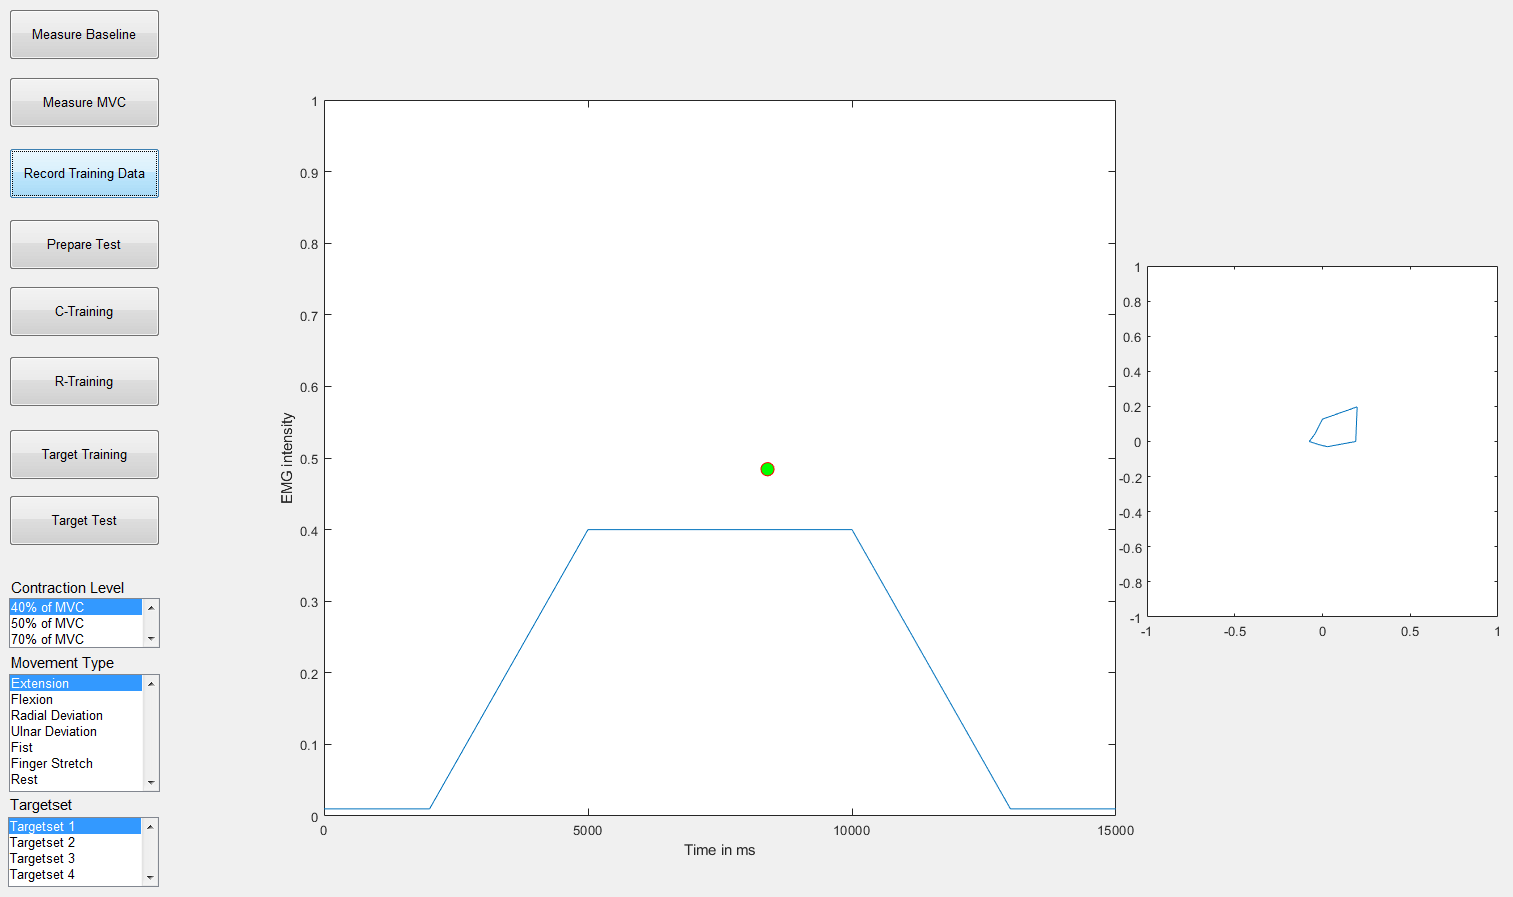
\includegraphics[width=1\textwidth]{figures/xBackground/dataacqGUI}
	\caption{The implemented data acquisition interface. On the left is different buttons shown, where only "Measure Baseline", "Measure MVC" and "Record Training Data" is used in the data acquisition. The "Contraction Level" menu forms the trapezoidal trajectory and "Movement Type" saves the performed movement the correct label. In the center is the trapezoidal trajectory and the cursor representing the EMG signal. On the right is the spider-plot used to evaluate the quality of the performed movement.}
	\label{fig:GUIplot}
\end{figure}
